\documentclass{beamer}

\usetheme{Madrid}      % 内置主题(推荐新手使用)
\useoutertheme{miniframes} % 外层主题:横向小方块目录条
% \usetheme{Frankfurt}
% \usepackage[x11names]{xcolor}  % 加载扩展色库
% \usecolortheme[named=OliveDrab3]{structure}  % 柔和绿色

\title{Wavelet Transform for Image Processing}
\author{
\texorpdfstring{
Zhang Jinrui\thanks{alternative email:zhangjr1022@mails.jlu.edu.cn}
\\
He Jiashun
\\
Meng Jingyuan
\\
Jiang Zishen
\\
Mo Zian
}
{
Zhang Jinrui\thanks{alternative email:zhangjr1022@mails.jlu.edu.cn}
,
He Jiashun
,
Meng Jingyuan
,
Jiang Zishen
,
Mo Zian
}
}
\date{\today}

\begin{document}

\frame{\titlepage}  % 首页封面

\section{Pre-Processing}
\begin{frame}
    \frametitle{Pre}

    To transform a image into \(2^N \times 2^N\)

    sadfsa
    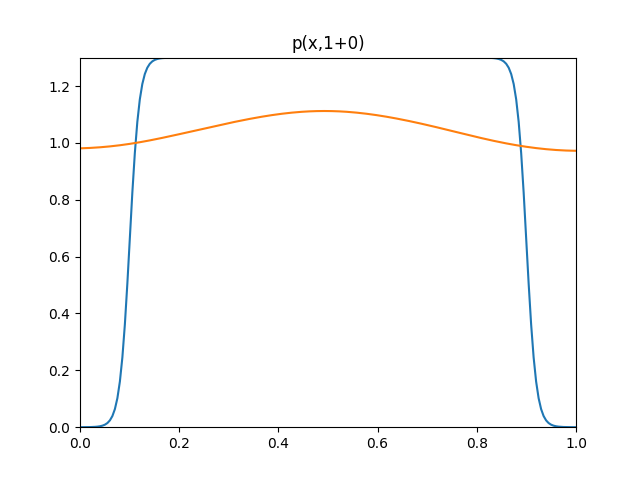
\includegraphics[width=0.5\textwidth]{fig/p(x,1+0).png}
    \pause

    sdfas
    \[
        E = mc^2
    \]
\end{frame}

\begin{frame}
    \frametitle{sadf}
    \begin{itemize}[<+->]
        \item sadf
        \item sadf
        \item sdgas
    \end{itemize}
\end{frame}

\begin{frame}
    \frametitle{Basic Idea}
    Vector decomposition.
\end{frame}

\section{Haar Compression}
\begin{frame}
    \frametitle{Standard Haar Decomposition}
    \begin{itemize}
        \item sdlfkj
        \item sDF
        \item sdf
    \end{itemize}
\end{frame}
\begin{frame}
    \frametitle{sfdfg}
    \begin{itemize}
        \item sdlfkj
        \item sDF
        \item sdf
    \end{itemize}
\end{frame}
\begin{frame}
    \frametitle{sadsgkjh}
    \begin{itemize}
        \item sdlfkj
        \item sDF
        \item sdf
    \end{itemize}
\end{frame}
\begin{frame}
    \frametitle{sdf}
    \begin{itemize}
        \item sdlfkj
        \item sDF
        \item sdf
    \end{itemize}
\end{frame}

\section{Haar Compression Augmented}
\begin{frame}
    \frametitle{Basic Idea}
    \begin{itemize}
        \item \[
                  \sum_{k=1}^{n}\hat{l}_k^4
                  \leq
                  (\sum_{k=1}^{n}\hat{l}_k^2)^2
                  =
                  (\sum_{k=1}^{n}l_k^2)^2
              \]
        \item \[
                  \min_{\hat{l}_k\in l^2 st. \sum_{k=1}^{n}\hat{l}_k^2=\sum_{k=1}^{n}l_k^2}(-\sum_{k=1}^{n}\hat{l}_k^4)
              \]
    \end{itemize}
\end{frame}
\begin{frame}
    \frametitle{Basic Idea}
    \begin{itemize}
        \item 	\begin{figure}
                  \centering
                  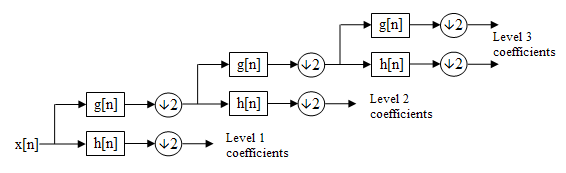
\includegraphics[width=0.8\textwidth]{fig/Wavelets_-_Filter_Bank.png}
                  \caption{Cascading}
                  \label{fig:Cascading}
              \end{figure}
        \item \[
                  \min_{\Phi}(-\sum_{k=1}^{n}\hat{l}_k^4)
              \]
        \item Condense the energy to as less coefficients as possible.
    \end{itemize}
\end{frame}
\begin{frame}
    \frametitle{Results}
    \begin{itemize}
        \item
              \begin{figure}[ht!]
                  \centering
                  \begin{minipage}{0.45\textwidth}
                      \centering
                      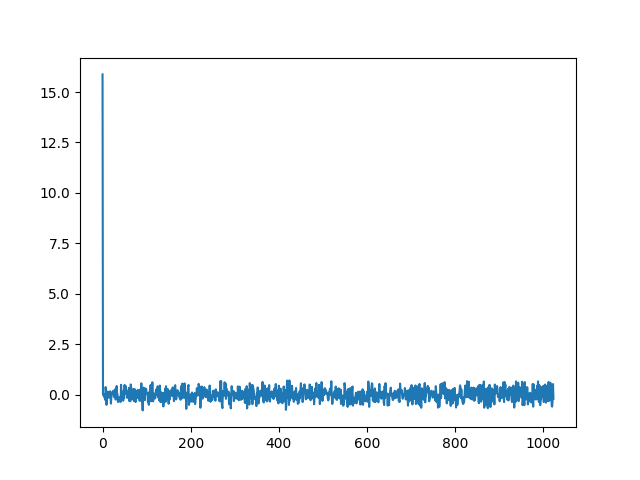
\includegraphics[width=0.9\textwidth]{fig/HaarAugmented1D_freq.png} % first figure itself
                      \caption{Haar 2x2 filter bank random input. Compression Rate 0.2568}
                      \label{fig:Haar}
                  \end{minipage}\hfill
                  \begin{minipage}{0.45\textwidth}
                      \centering
                      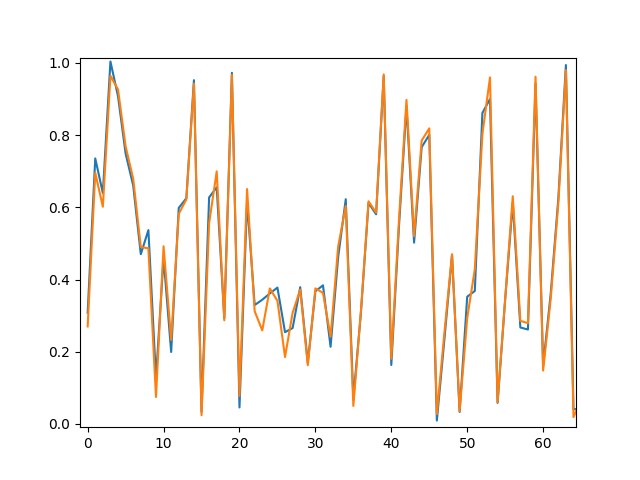
\includegraphics[width=0.9\textwidth]{fig/HaarAugmented1D_rec.png} % second figure itself
                      \caption{Haar 2x2 filter bank random input.Total average energy loss 0.0009}
                  \end{minipage}
              \end{figure}
              %   \begin{figure}
              %       \centering
              %       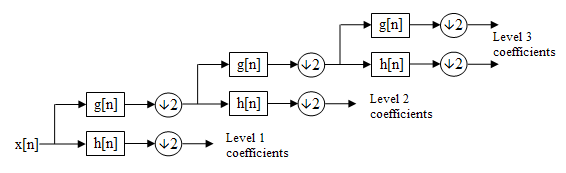
\includegraphics[width=0.8\textwidth]{fig/Wavelets_-_Filter_Bank.png}
              %       \caption{Siakam won 2025 NBA eastern conference finals MVP}
              %       \label{fig:Siakam}
              %   \end{figure}
        \item random sequence would take more information entropy so have a low compress rate.
    \end{itemize}
\end{frame}
\begin{frame}
    \frametitle{Results}
    \begin{itemize}
        \item
              \begin{figure}[ht!]
                  \centering
                  \begin{minipage}{0.45\textwidth}
                      \centering
                      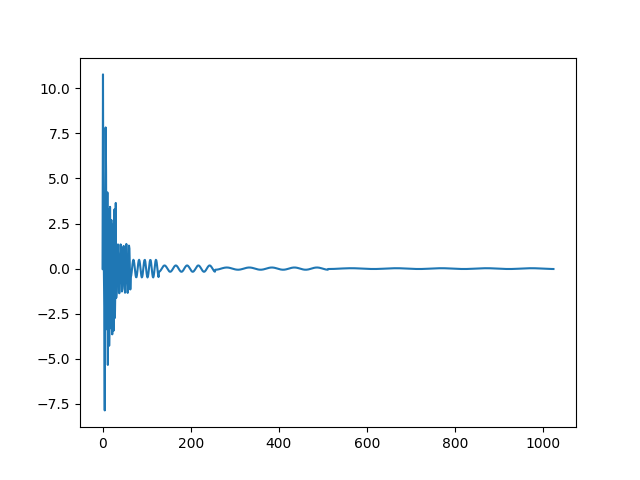
\includegraphics[width=0.9\textwidth]{fig/HaarAugmented1D_sin_freq.png} % first figure itself
                      \caption{Haar 2x2 filter bank sin input frequency. Compression Rate 0.9287}
                      \label{fig:Haar_sin}
                  \end{minipage}\hfill
                  \begin{minipage}{0.45\textwidth}
                      \centering
                      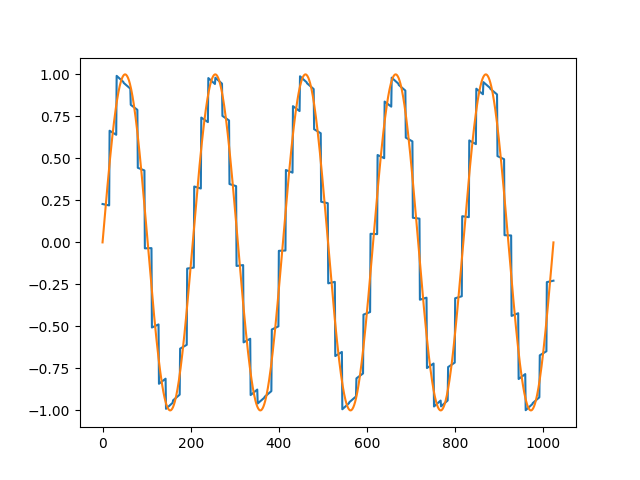
\includegraphics[width=0.9\textwidth]{fig/HaarAugmented1D_sin_rec.png} % second figure itself
                      \caption{Haar 2x2 filter bank sin input reconstruction.Total average energy loss 0.0104}
                  \end{minipage}
              \end{figure}
              %   \begin{figure}
              %       \centering
              %       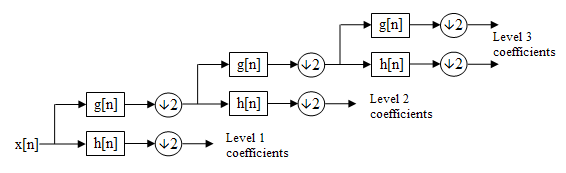
\includegraphics[width=0.8\textwidth]{fig/Wavelets_-_Filter_Bank.png}
              %       \caption{Siakam won 2025 NBA eastern conference finals MVP}
              %       \label{fig:Siakam}
              %   \end{figure}
        \item a smooth signal not have much information entropy, so will have a high compress rate.
    \end{itemize}
\end{frame}
\begin{frame}
    \frametitle{Results}
    \begin{itemize}
        \item
              \begin{figure}[ht!]
                  \centering
                  \begin{minipage}{0.45\textwidth}
                      \centering
                      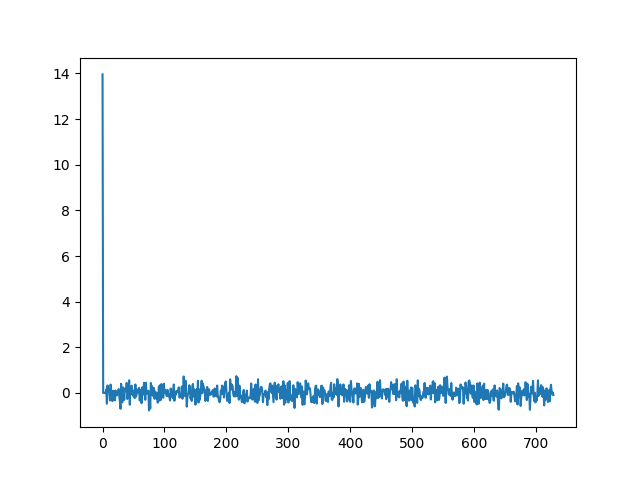
\includegraphics[width=0.9\textwidth]{fig/Haar3Augmented1D_freq.png} % first figure itself
                      \caption{Haar 3x3 filter bank random input. Compression Rate 0.1906}
                      \label{fig:Haar3}
                  \end{minipage}\hfill
                  \begin{minipage}{0.45\textwidth}
                      \centering
                      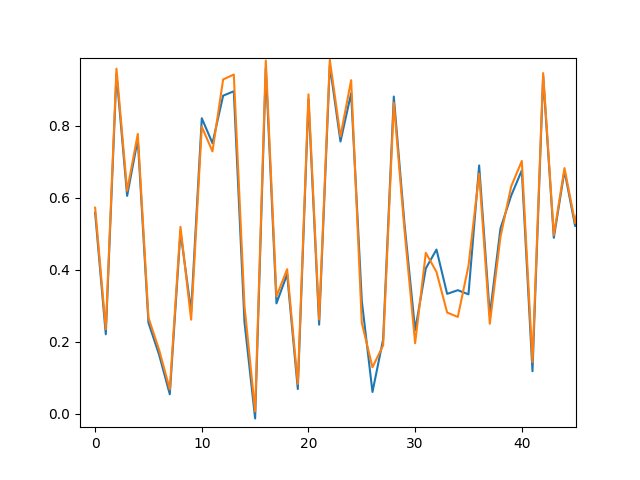
\includegraphics[width=0.9\textwidth]{fig/Haar3Augmented1D_rec.png} % second figure itself
                      \caption{Haar 3x3 filter bank random input.Total average energy loss 0.0008}
                  \end{minipage}
              \end{figure}
              %   \begin{figure}
              %       \centering
              %       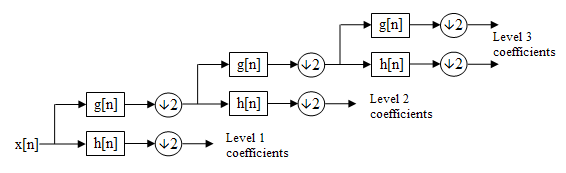
\includegraphics[width=0.8\textwidth]{fig/Wavelets_-_Filter_Bank.png}
              %       \caption{Siakam won 2025 NBA eastern conference finals MVP}
              %       \label{fig:Siakam}
              %   \end{figure}
        \item same random sequence same reason.
    \end{itemize}
\end{frame}
\begin{frame}
    \frametitle{Results}
    \begin{itemize}
        \item
              \begin{figure}[ht!]
                  \centering
                  \begin{minipage}{0.45\textwidth}
                      \centering
                      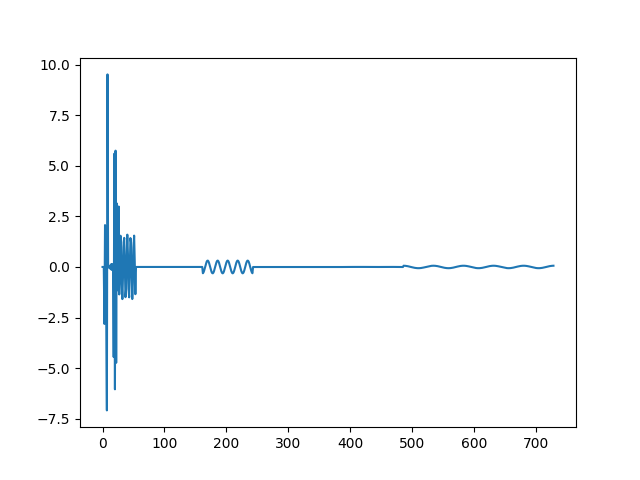
\includegraphics[width=0.9\textwidth]{fig/Haar3Augmented1D_sin_freq.png} % first figure itself
                      \caption{Haar 3x3 filter bank sin input frequency. Compression Rate 0.7750}
                      \label{fig:Haar3_sin}
                  \end{minipage}\hfill
                  \begin{minipage}{0.45\textwidth}
                      \centering
                      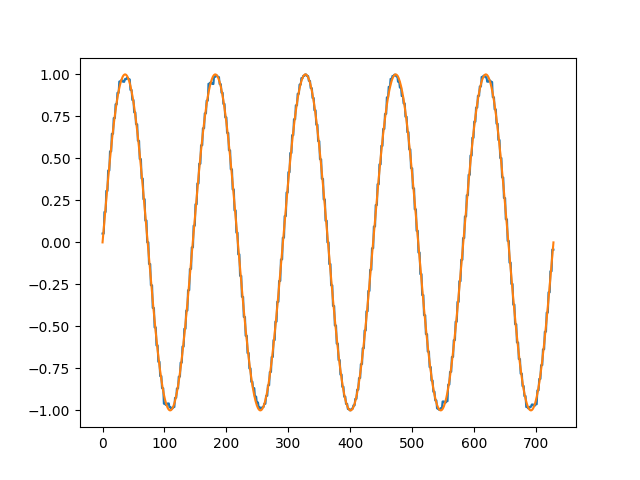
\includegraphics[width=0.9\textwidth]{fig/Haar3Augmented1D_sin_rec.png} % second figure itself
                      \caption{Haar 3x3 filter bank sin input reconstruction.Total average energy loss 0.0007}
                  \end{minipage}
              \end{figure}
              %   \begin{figure}
              %       \centering
              %       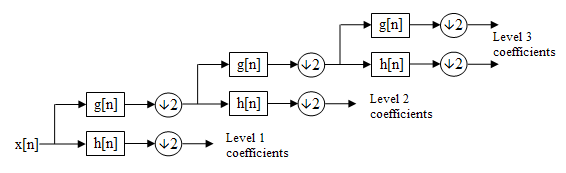
\includegraphics[width=0.8\textwidth]{fig/Wavelets_-_Filter_Bank.png}
              %       \caption{Siakam won 2025 NBA eastern conference finals MVP}
              %       \label{fig:Siakam}
              %   \end{figure}
        \item same smooth signal same reason.
    \end{itemize}
\end{frame}

\section{Zishen Jiang}
\begin{frame}
    \frametitle{sadsgkjh}
    \begin{itemize}
        \item sdlfkj
        \item sDF
        \item sdf
    \end{itemize}
\end{frame}

\section{Energy Analysis}
\begin{frame}
    \frametitle{sdf}
    \begin{itemize}
        \item sdlfkj
        \item sDF
        \item sdf
    \end{itemize}
\end{frame}

\end{document}
